\documentclass[aspectratio=169]{beamer}
\usetheme{Madrid}
\usecolortheme{beaver}

\usepackage[UTF8,fontset=fandol]{ctex}
\usepackage{amsmath, amssymb}
\usepackage{booktabs}
\usepackage{ragged2e}
\usepackage{array}
\newcommand{\framebottomnote}[1]{%
    \vfill
    \par\noindent
    {\tiny\color{black!65}\parbox{0.96\linewidth}{#1}\par}%
    \vspace*{-0.75cm}%
}

\title[report]{进展汇报}
\date{2026-03-25}

\begin{document}

\begin{frame}
    \titlepage
\end{frame}

\section{问题收敛与目标}

\begin{frame}{研究重点}
    \begin{center}
        \Large \textbf{helplessness}
    \end{center}
    \vspace{0.15cm}
    \begin{itemize}
        \item \textbf{任务 $\rightarrow$ 反馈 $\rightarrow$ helplessness 更新 $\rightarrow$ 后续行为}
        \item 重点考察 support 是否能够缓冲 helplessness 的累积
    \end{itemize}
\end{frame}

\section{文献依据}

\begin{frame}{为什么聚焦 helplessness}
    \begin{itemize}
        \item 个体在反复经历不可控压力与失败后，无助感会逐步增强
        \item 这类研究通常将 \textbf{控制感下降} 与 \textbf{后续努力意愿下降} 联系起来分析
        \item 因此，将 helplessness 设为核心状态变量，具有较明确的理论依据
        \item helplessness 不是被摩擦本身更新的，而是由任务之后个体到底觉得“我努力有用”还是“我努力没用”来更新的
    \end{itemize}
    \framebottomnote{参考文献：Tafet and Ortiz Alonso, learned helplessness and learned controllability, \textit{Frontiers in Psychiatry}, 2025-08-26。}
\end{frame}

\begin{frame}{为什么保留 support、self-efficacy、anxiety}
    \begin{itemize}
        \item \textbf{technology anxiety} 会影响后续数字使用意愿
        \item \textbf{self-efficacy} 与 \textbf{perceived usefulness} 也会显著影响持续使用倾向
        \item \textbf{family support} 与 \textbf{formal support} 并非边缘因素，它们与使用意愿及技术恐惧均有关联
    \end{itemize}
    \framebottomnote{参考文献：An et al., older adults' self-perception, technology anxiety, and intention to use digital public services, \textit{BMC Public Health}, 2024-12-19；Jokisch et al., acceptance of digital health services among older adults, \textit{Frontiers in Public Health}, 2022-12-13。\\Han et al., influencing factors of digital health technology anxiety in the elderly, \textit{Frontiers in Psychology}, 2025-10-02；Song et al., technophobia in digital health contexts, \textit{DIGITAL HEALTH}, 2025-09-02。\\Sun et al., factors that influence technophobia in Chinese older patients with ischemic stroke, \textit{BMC Geriatrics}, 2025-08-19。}
\end{frame}

\begin{frame}{相对 AgentSociety 的修改}
    \begin{itemize}
        \item 将原本面向一般社会生活模拟的 agent，改为面向数字摩擦场景的 agent
        \item 将自由度较高的生成式决策流程，改为规则和 LLM 共同参与的决策方法
        \item 将自由式 interview 改为结构化解释输出，便于分析与状态回写
    \end{itemize}
\end{frame}

\section{框架定位}

\begin{frame}{模型机制设计}
    \begin{center}
        \Large \textbf{规则与 LLM 融合，暂以规则主导}
    \end{center}
    \vspace{0.15cm}
    \begin{itemize}
        \item \textbf{沿用 AgentSociety 的部分：} workflow、survey/interview、agent 外层结构
        \item \textbf{本工作重点改造的部分：} 围绕 helplessness 的状态更新与行为链条
        \item \textbf{功能分工：} 规则决定 outcome 与主状态更新，LLM 负责任务理解、策略权衡与主观解释
    \end{itemize}
\end{frame}

\begin{frame}{核心机制链}
    \centering
    \includegraphics[width=\textwidth,height=0.82\textheight,keepaspectratio]{/Users/pifazuoren/Desktop/ph1.png}
\end{frame}

\begin{frame}{LLM 的作用位置}
    \begin{enumerate}
        \item \textbf{任务判断：} 形成 task appraisal
        \item \textbf{策略选择：} 在自行尝试、求助、回避之间做有限权衡
        \item \textbf{主观输出：} 生成 survey 与 interview 中的解释性内容
    \end{enumerate}
    \vspace{0.15cm}
    \begin{center}
        \large \textbf{success / failure 与 helplessness 的主要更新，仍由规则机制决定}
    \end{center}
\end{frame}

\section{当前实验}

\begin{frame}{实验设置}
    \begin{itemize}
        \item 当前展示结果来自 4 个实验条件与 1 组 seed（101）
        \item 每个条件包含 10 个 agents
        \item \texttt{full} 多阶段设置为：\texttt{steady $\rightarrow$ shock $\rightarrow$ recovery}
        \item 每个 stage 持续 2 天，决策步长为 30 分钟
        \item 当前启用 Phase 1、Phase 2 与 Phase 5
    \end{itemize}
\end{frame}

\begin{frame}{当前结果的解释边界}
    \begin{itemize}
        \item 本次运行 \textbf{未完整覆盖全部三个 stages}
        \item 但 4 个条件均完整完成了第 1 个 stage：\texttt{steady}
        \item 中断位置发生在 Phase 5 的 interview readback 环节
        \item 因而当前结果应视为 \textbf{steady 阶段的初步观察}
    \end{itemize}
\end{frame}

\begin{frame}{Steady 阶段：行为分布}
    \centering
    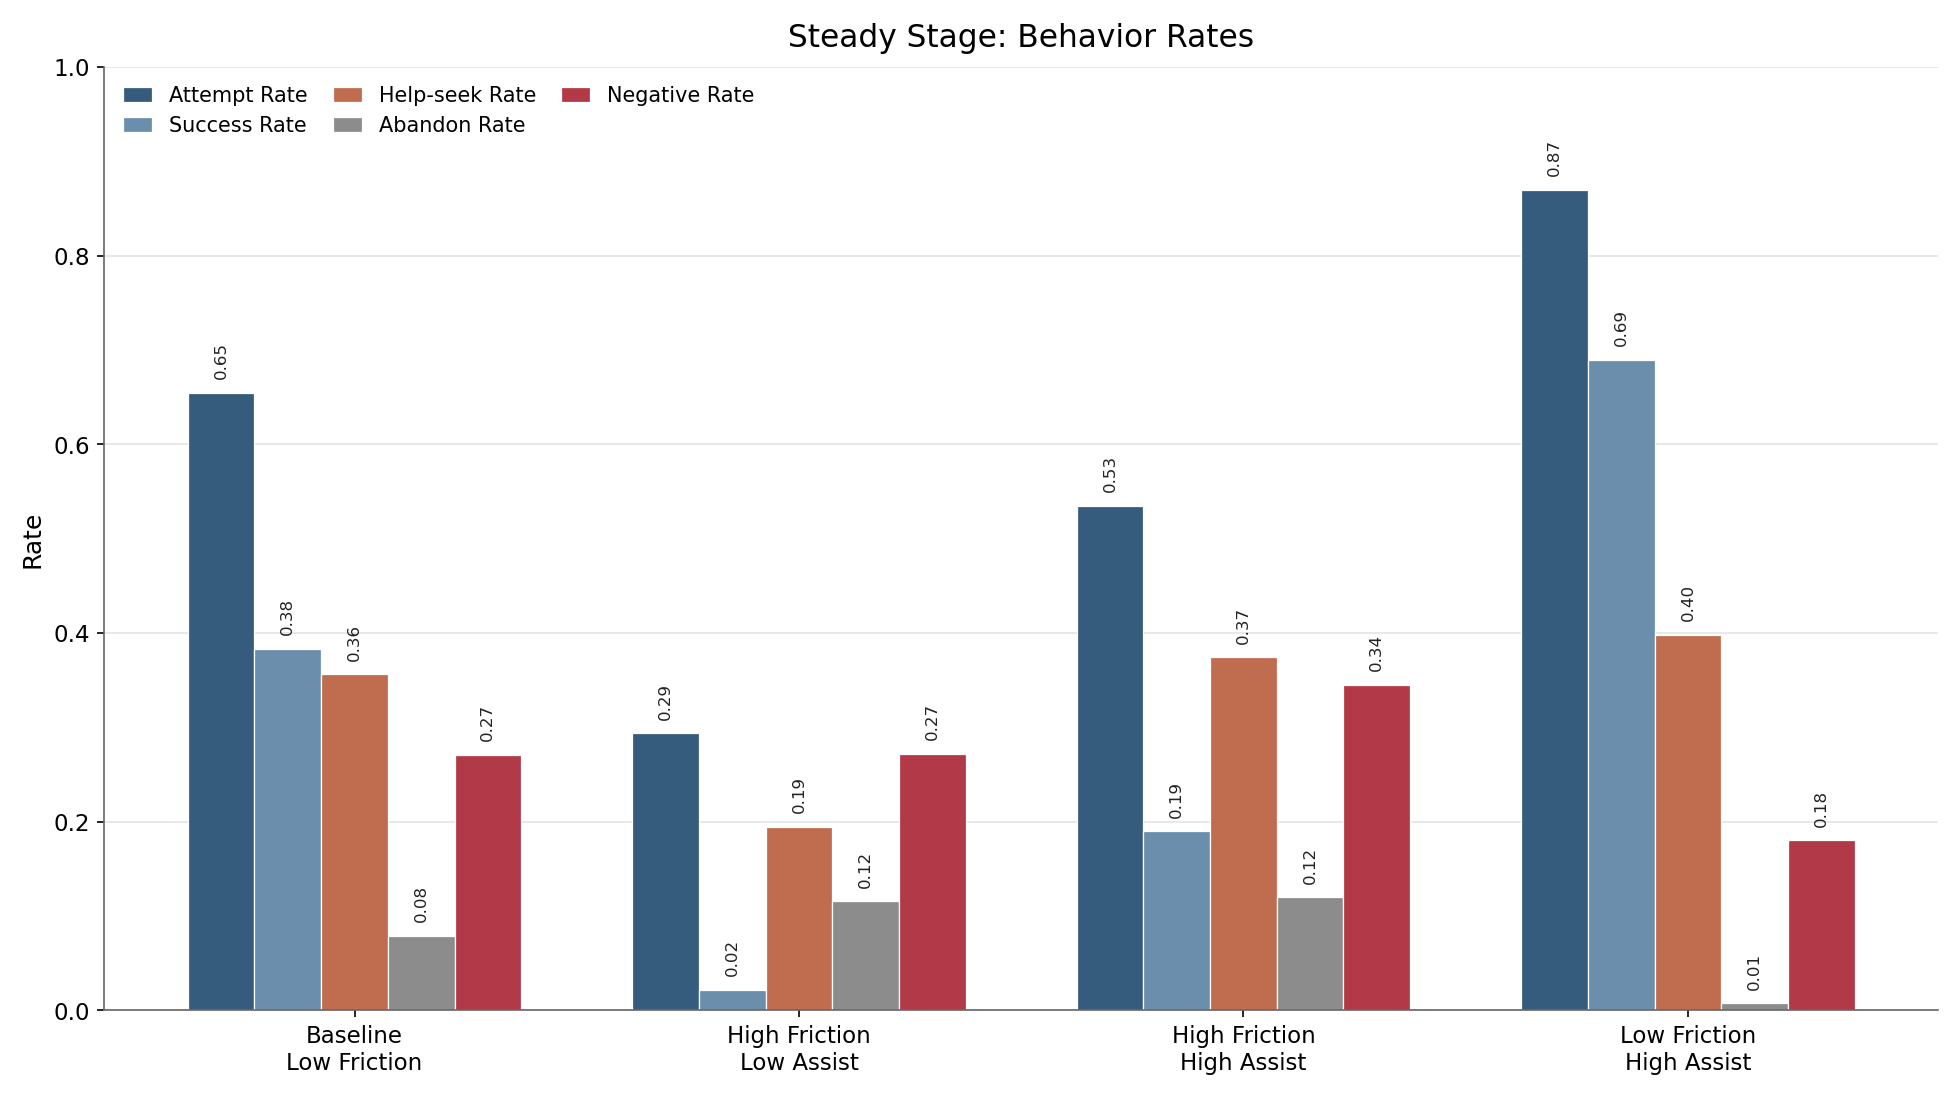
\includegraphics[width=\textwidth,height=0.82\textheight,keepaspectratio]{examples/digital_friction_mvp/analysis/report0325_figures/steady_behavior_rates.png}
\end{frame}

\begin{frame}{Steady 阶段：Helplessness 变化幅度}
    \centering
    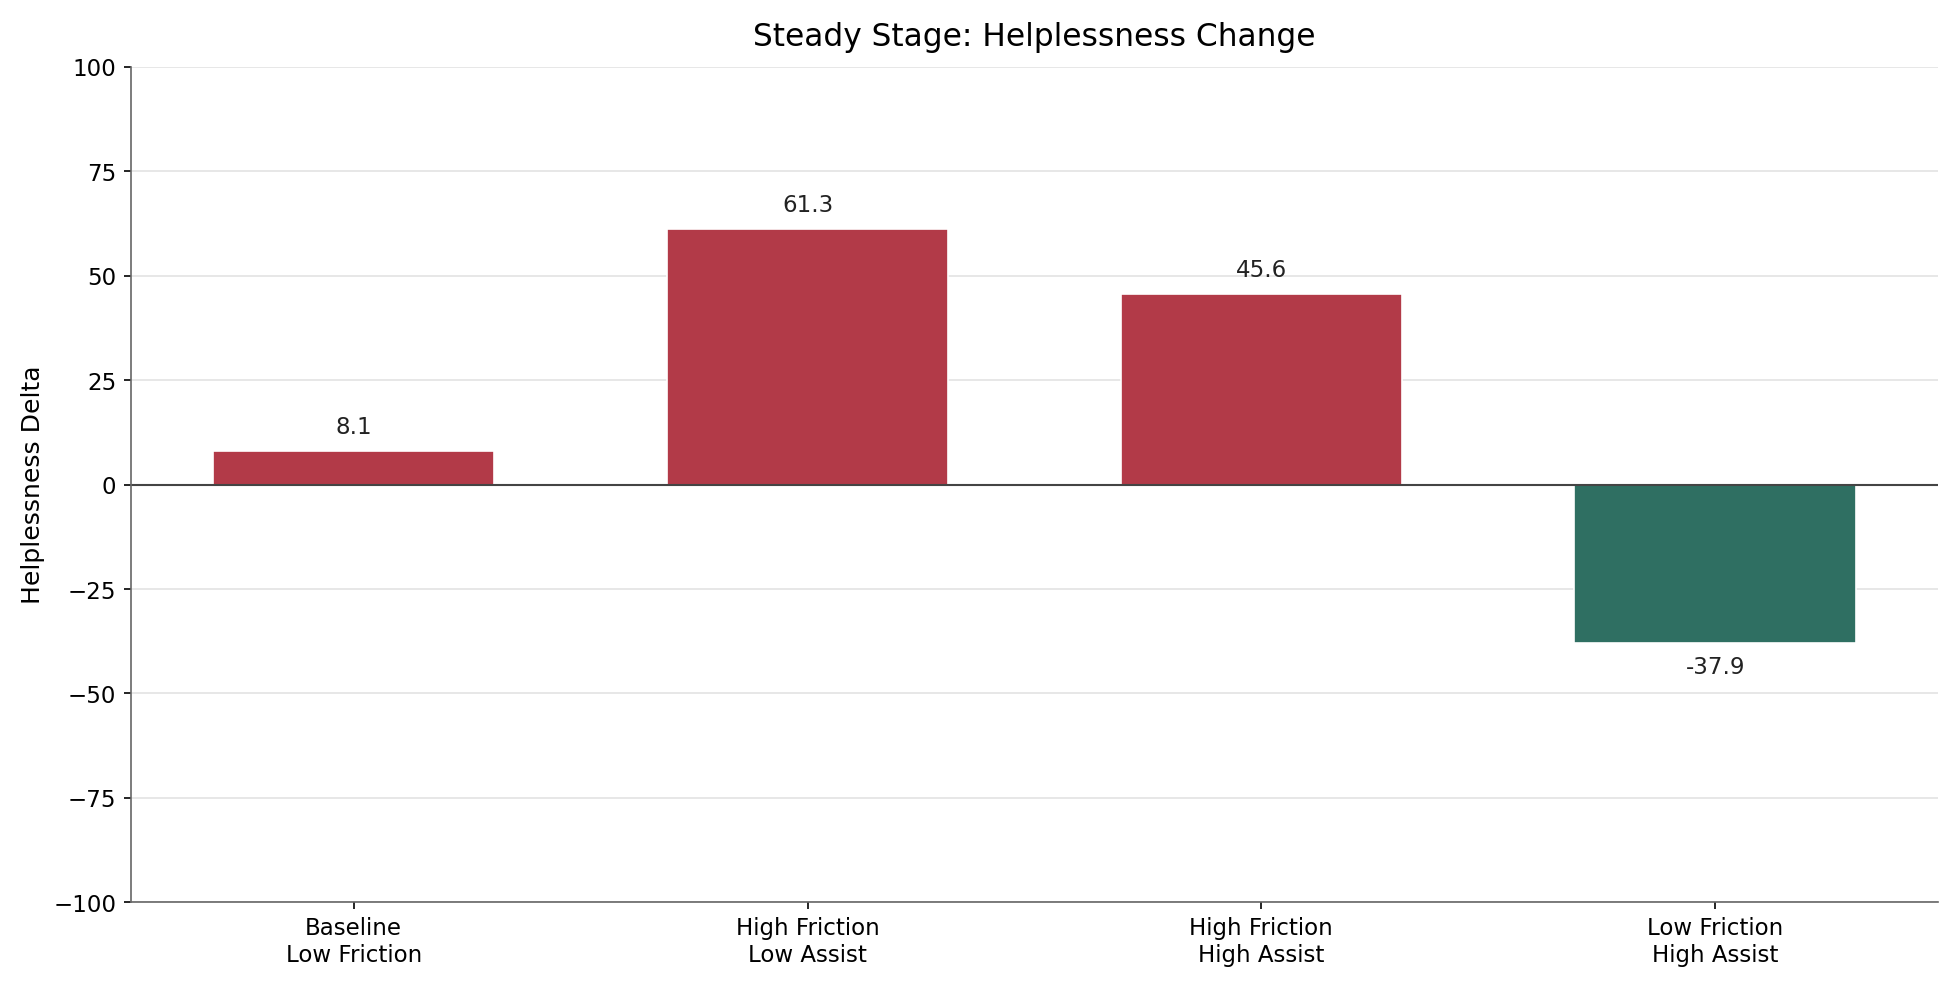
\includegraphics[width=\textwidth,height=0.82\textheight,keepaspectratio]{examples/digital_friction_mvp/analysis/report0325_figures/steady_helplessness_delta.png}
\end{frame}

\begin{frame}{当前可以支持的结论}
    \begin{itemize}
        \item \textbf{表现最优的条件：} low friction + high assist
        \item \textbf{表现最弱的条件：} high friction + low assist
        \item \textbf{介于其间的条件：} high friction + high assist
    \end{itemize}
    \vspace{0.15cm}
    \begin{center}
        \Large \textbf{friction 与 support 的组合，会显著改变 helplessness 的累积方向}
    \end{center}
    \vspace{0.15cm}
    \begin{itemize}
        \item support 具有明确的缓冲作用
        \item 但目前仍不足以完全抵消高 friction 带来的负向影响
    \end{itemize}
\end{frame}

\section{当前问题与下一步}

\begin{frame}{还待完善的部分}
    \begin{itemize}
        \item \textbf{第一，证据稳定性仍不足：} 当前只有 single seed，且 full-run 中断
        \item \textbf{第二，机制论证仍需加强：} helplessness 的更新规则还需要更充分的理论与参数依据
    \end{itemize}
\end{frame}

\begin{frame}{下一步工作}
    \begin{itemize}
        \item 扩展 seeds，提高结果稳定性
        \item 在当前 hybrid 基础上，逐步增强 LLM 在任务理解、状态建模与策略生成中的作用
        \item 汇报与论文主线继续围绕：\textbf{friction $\rightarrow$ helplessness $\rightarrow$ behavior}
    \end{itemize}
\end{frame}

\begin{frame}
    \centering
    \Huge{请老师批评指正}
\end{frame}

\end{document}
